\documentclass[a4paper, 12pt]{article}
\usepackage[top=1cm, bottom=1.5cm, left=1cm, right=1cm]{geometry}
\usepackage[utf8]{inputenc}
\usepackage{graphicx, caption}
\usepackage{float}
\usepackage{amsmath, amsfonts, amssymb, esint}
\usepackage{multicol}
\usepackage{titlesec}
\usepackage{hyperref}
\usepackage{indentfirst}

\pagenumbering{Roman}

\titleformat{\section}{\normalfont\bfseries}{\thesection.}{0.5em}{}

\hypersetup
{
    colorlinks=true,
    linkcolor=blue,
    filecolor=magenta,      
    urlcolor=blue,
}

\begin{document}
	\begin{center}
	\begin{large}
		\textbf{Determinação da Viscosidade do Ar}	
	\end{large}
	\end{center}
	
	\begin{center}
		\textit{Iago Braz Mendes, Hugo Danilo Santos Alkimim, Gabriel Oliveira Mota, e Marcos Aurélio Duarte Carvalho}
	\end{center}

	\section*{Resumo}
		Neste artigo, explora-se um arranjo experimental de um oscilador massa-mola para investigar a oscilação harmônica amortecida. A determinação da amplitude da oscilação como uma função temporal foi determinada precisa e economicamente, utilizando vídeos obtidos por meio de um celular, a ferramenta \textit{Tracker -- Video Analysis and Modeling Tool for Physics Education --} e algoritmos em \textit{MATLAB}. Assim, foi possível determinar o coeficiente de amortecimento, que foi usado para encontrar a viscosidade do ar.

	\begin{multicols}{2}
		\setlength{\parindent}{4ex}
		\section{Introdução}
			\par A teoria acerca de sistemas oscilatórios amortecidos é aprofundada por alguns artigos [\textit{referência(s)}]. Contudo, é comum encontrar discrepâncias entre as previsões e os resultados obtidos em laboratórios. Nesse sentido, este artigo apresenta um modelo experimental de fácil implementação para determinar a viscosidade do ar a partir de uma oscilação massa-mola amortecida. Com os dados coletados, fazemos 3 análises a fim de encontrar qual método mais se aproxima da realidade.
			\par Na seção \hyperref[sec:teoria]{\ref{sec:teoria}}, a parte teórica sobre viscosidade e oscilações amortecidas é rapidamente exposta. Na seção \hyperref[sec:experimento]{\ref{sec:experimento}}, o modelo experimental usado para obter dados é explicado. Na seção \hyperref[sec:analise]{\ref{sec:analise}}, a análise de dados e seus resultados são discutidos, abrangendo 3 métodos distintos. Por fim, as conclusões são apresentadas na seção \hyperref[sec:conclusao]{\ref{sec:conclusao}}.
			
		\section{Teoria} \label{sec:teoria}
			\par Em primeira instância, viscosidade ($\eta$) é a propriedade física que descreve a resistência de um fluido para escoar, que é geralmente expressa usando a Lei de Newton da Viscosidade:
			\begin{figure}[H]
				\centering
				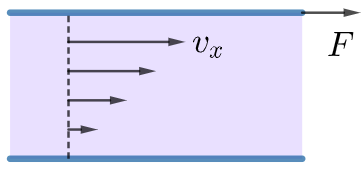
\includegraphics[scale=0.6]{./img/viscosidade.png}
			\end{figure}
			\begin{equation}
				\frac{F}{A} = \eta \dfrac{dv_x}{dy}
			\end{equation}
			em que $F$ é a força aplicada, $A$ é a área em $y$ e $z$, e $\dfrac{dv_x}{dy}$ é a derivada espacial da velocidade. No Sistema Internacional, a viscosidade possui \textit{pascal-segundo} [$Pa \cdot s$] como unidade de medida.
			\par Além disso, quando estudamos a mecânica de fluidos, devemos sempre considerar o número de Reynolds, um coeficiente adimensional utilizado para o cálculo do regime de escoamento de um fluido sobre uma superfície. Esse coeficiente é dado por:
			\begin{equation}
				Re = \frac{\rho v l}{\eta}
			\end{equation}
			em que $\rho$ é a densidade do fluido e $l$ é a dimensão linear característica do objeto oscilante (para uma esfera, $l = 2 r$, em que $r$ é o raio).
			\par Finalmente, quando analizamos oscilações harmônicas simples no mundo real, precisamos considerar a energia dissipada devido à força de atrito. Para pequenos números de Reynolds, a força de atrito na esfera é dada pela Lei de Stoke:
			\begin{equation}
				F = 6 \pi r \eta v
			\end{equation}
			\par Nesse caso, a equação do movimento para uma esfera com massa $m$ e uma mola com constante elástica $k$ é dada por
			\begin{equation}
				\ddot{x} + 2 \gamma \dot{x} + \omega_0^2 x = 0
			\end{equation}
			em que as constantes são dadas por
			\begin{equation}
				\omega_0^2 = \frac{k}{m} \qquad \gamma = \frac{3 \pi \eta r}{m}
			\end{equation}
			\par Portanto, quando $\omega_0 > \gamma$ (caso de sub-amortecimento), a solução é
			\begin{equation}
				x = A \, e^{- \gamma t} \, \cos (\omega t + \phi)
			\end{equation}
			em que $A$, $\phi$ e $\omega$ são, respectivamente, a amplitude, a fase, e a frequência da oscilação.
			\par Contudo, quando os números de Reynolds não são pequenos, podemos usar a equação desenvolvida por Landau e Lifshitz:
			\small \begin{equation} \label{eq:landau}
				F = 6 \pi \eta r \left(1 + \frac{r}{\delta} \right) v + 3 \pi r^2 \left( 1 + \frac{2 r}{9 \delta} \right) \rho \delta \dfrac{d v}{d t}
			\end{equation} \normalsize
			em que $\delta$ a profundidade de penetração dentro do fluido ao redor do objeto oscilante, que é dada por
			\begin{equation}
				\delta = \sqrt{\frac{2 \eta}{\rho \omega}}
			\end{equation}
			\par Quando resolvemos essa equação, encontramos uma solução análoga à anterior:
			\begin{equation} \label{eq:posicao}
				x = A \, e^{- \gamma t} \, \cos (\omega t + \phi)
			\end{equation}
			\par Todavia, agora as constantes são determinadas por
			\begin{equation} \label{eq:constantes} \begin{split}
				\omega_0^2 = \frac{k}{f_2 3 \pi r^2 \left(1 + \frac{2 r}{9 \delta} \right) + m} \\
				\gamma = \frac{3 \pi \eta r \left(1+ \frac{r}{\delta} \right)}{f_1 \left[ f_2 3 \pi r^2 \left(1+\frac{2 r}{9 \delta} \right) \rho \delta + m \right]}
			\end{split} \end{equation}
			em que $f_1$ e $f_2$ são coeficientes semi-empíricos.
			\par Neste artigo, fazemos uso somente dos pontos máximos da oscilação (ou seja, das amplitudes). Com isso, a equação \hyperref[eq:posicao]{\ref{eq:posicao}} pode ser reescrita da seguinte forma:
			\begin{equation}
				A = A_0 e^{- \gamma t} \quad \therefore \quad \ln A = - \gamma t + \ln A_0
			\end{equation}
			em que $A$ é a amplitude em função do tempo e $A_0$ é a amplitude inicial.
			
		\section{Experimento} \label{sec:experimento}
			\par A configuração experimental é simples e pode ser facilmente repetida. Ela consiste de uma bola com uma massa conhecida, uma mola, um suporte com uma escala de comprimento, um dispositivo para gravar a oscilação, um suporte para o dispositivo, e um cronômetro.
			\par Inicialmente, fizemos o experimento usando uma bola de tênis (\hyperref[img:tenis]{Figura 1}) e filmamos toda a oscilação. Após analisar os dados dessa configuração, optamos por utilizar um objeto de estudo com menor rugosidade superficial, visando adequar nosso experimento aos modelos matemáticos utilizados. Além disso, optamos por gravar trechos mais curtos, a fim de obter vídeos que representem a oscilação em cada minuto, facilitando a análise de dados.
			\par Portanto, fizemos um segundo experimento usando uma bola de metal (figura \hyperref[img:metal]{Figura 2}) e filmamos entre 5 e 10 segundos em intervalos de 1 minuto.
			\par Por fim, uma terceira configuração foi estabelecida, em que o movimento amortecido de uma bola de metal (similar à \hyperref[img:metal]{Figura 2}) foi gravado num período de 30 minutos sem interrupções.
			\begin{figure}[H] \label{img:tenis}
				\centering
				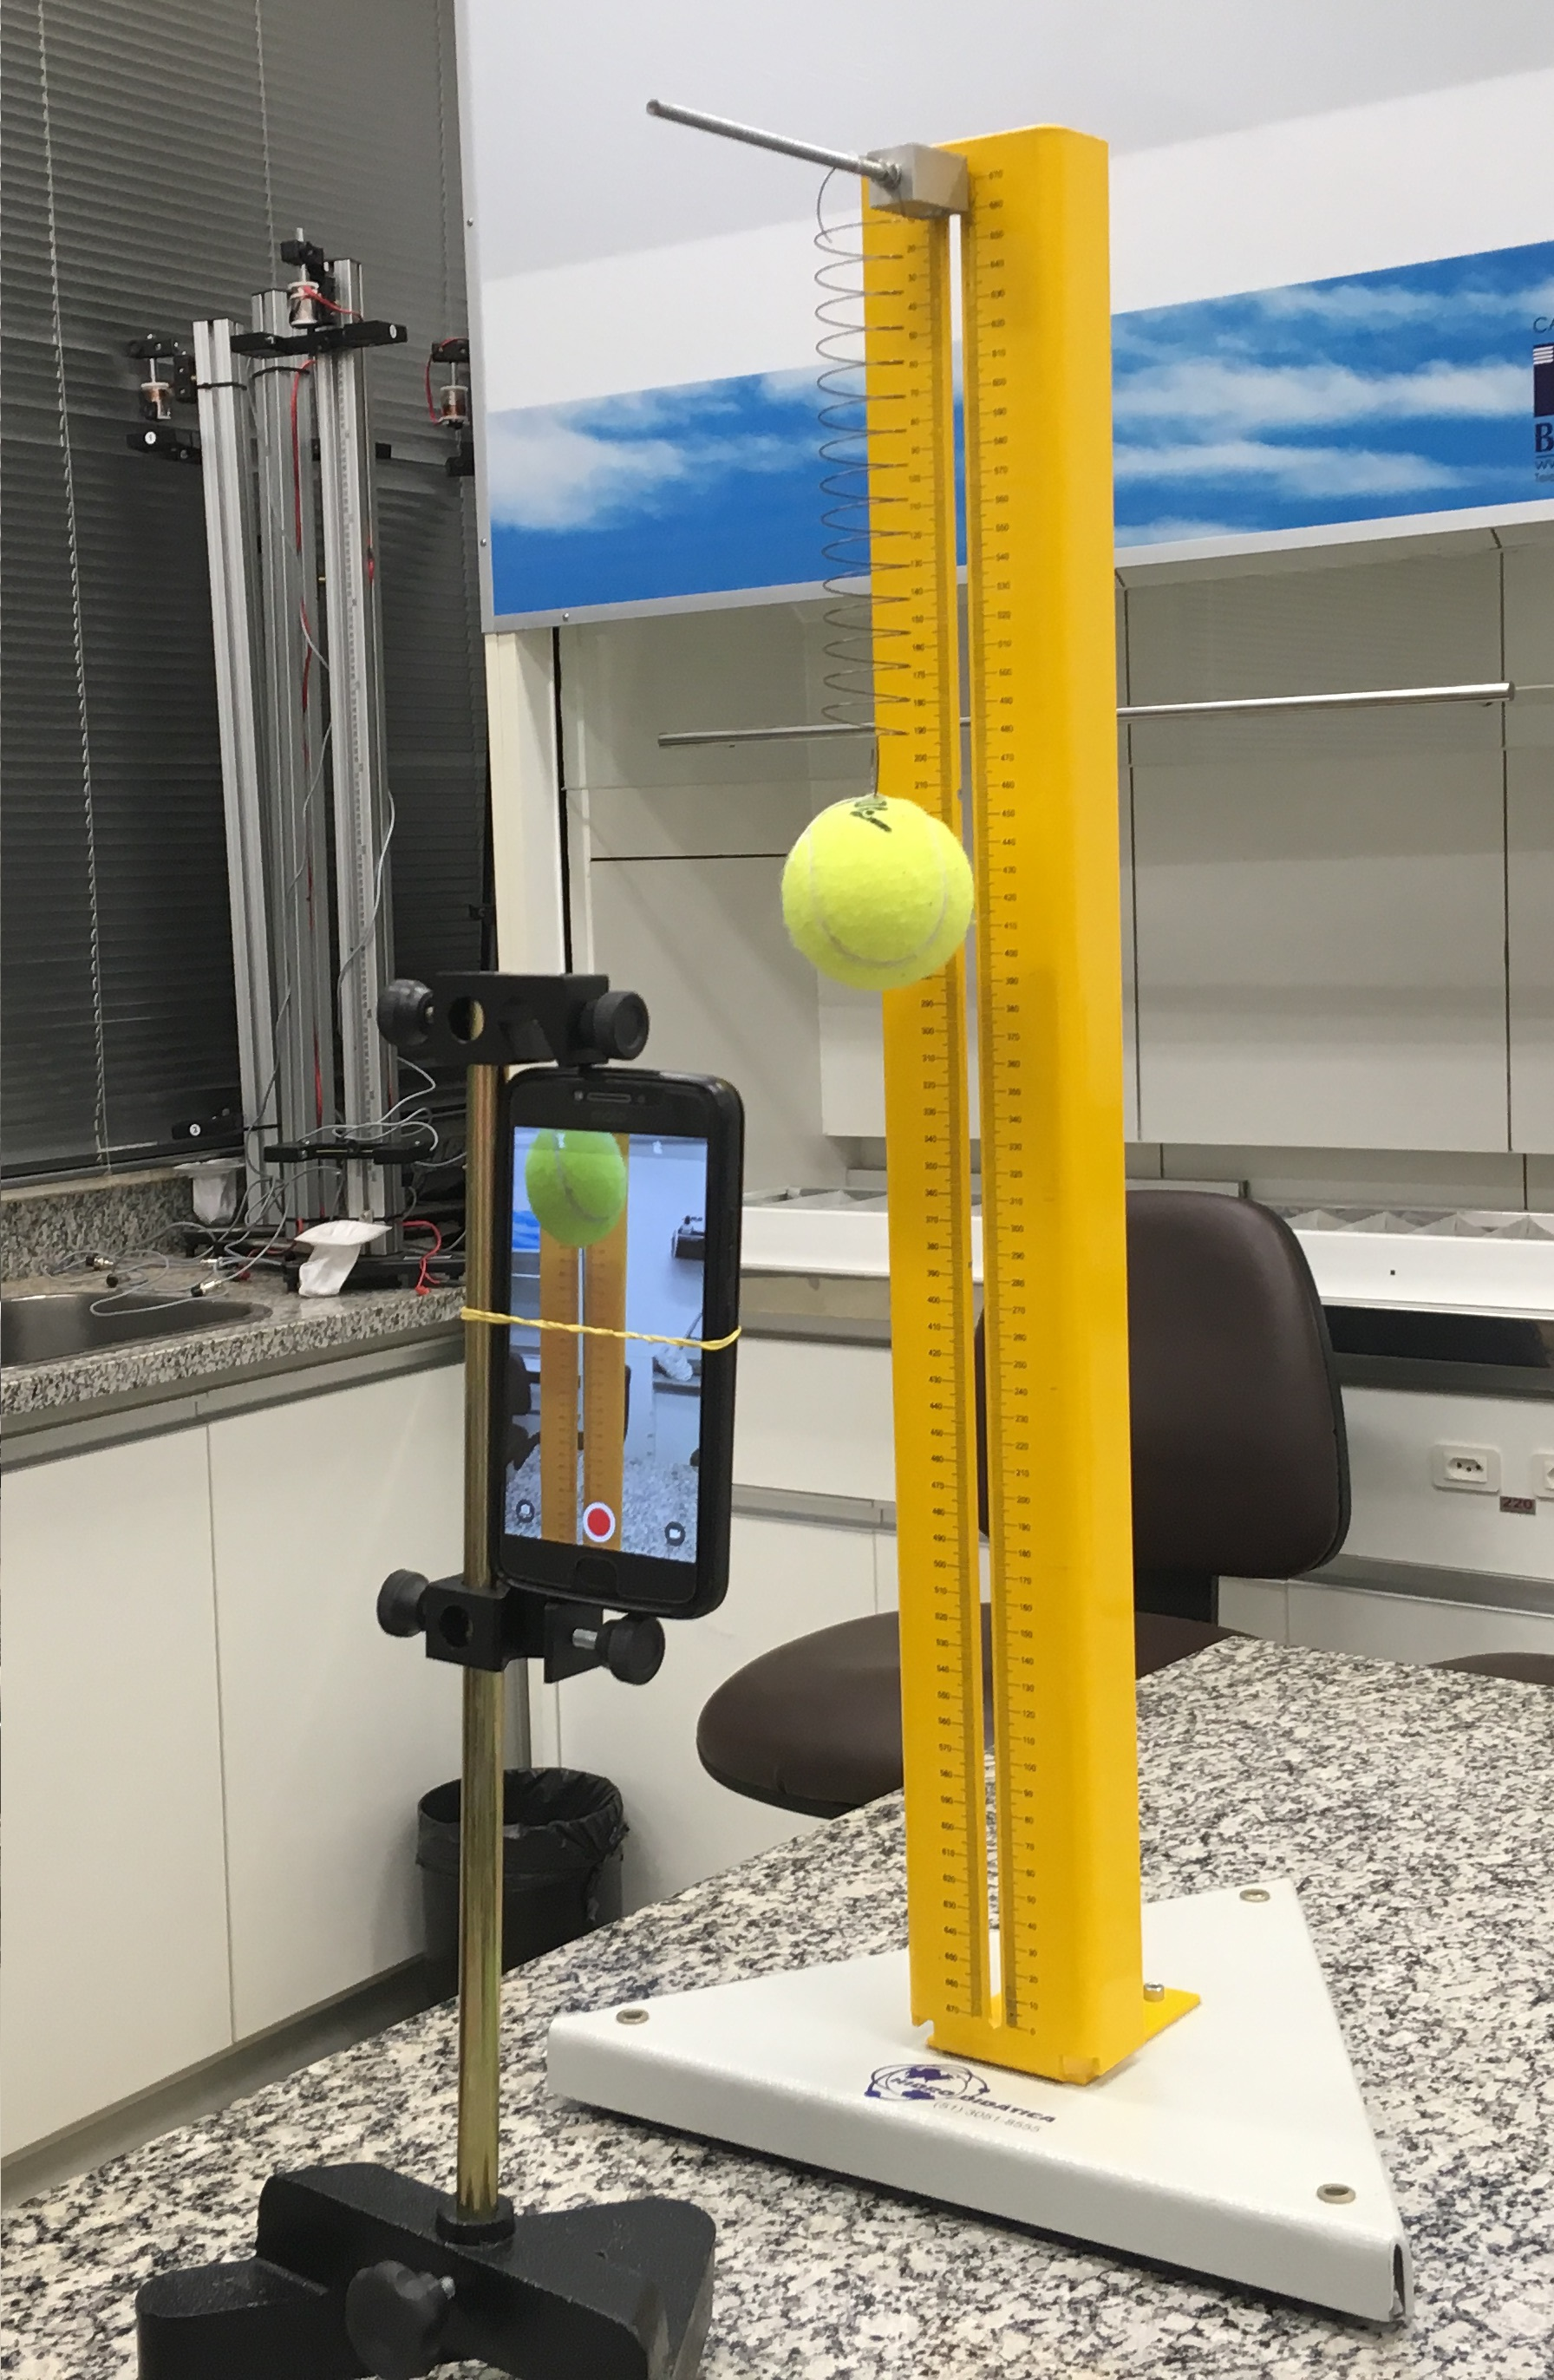
\includegraphics[scale=0.09]{./img/bolaTenis.jpg}
				\captionsetup{labelformat=empty}
				\caption{\textbf{Figura 1:} Experimento com bola de tênis.}
			\end{figure}
			\begin{figure}[H] \label{img:metal}
				\centering
				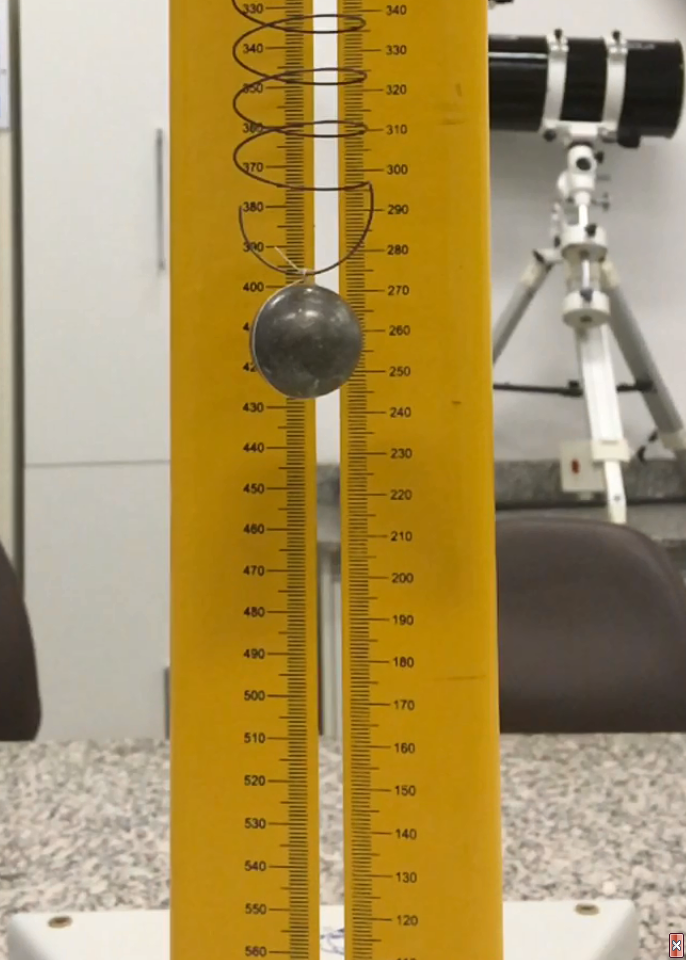
\includegraphics[scale=0.3]{./img/bolaMetal.png}
				\captionsetup{labelformat=empty}
				\caption{\textbf{Figura 2:} Experimento com bola de metal.}
			\end{figure}
			
		\section{Análise de Dados} \label{sec:analise}
			\par Com os dados da segunda configuração, fizemos três análises para determinar o valor da viscosidade do ar: utilizando a maior amplitude de cada vídeo curto e fazendo a média aritmética das amplitudes máxima e mínima em cada vídeo.
			\par No primeiro método, analisamos cada gravação -- quadro a quadro --, com o auxílio de um editor de vídeo (\hyperref[img:quadros]{Figura 3}), para encontrar a maior amplitude atingida e o correspondente tempo no cronômetro em tela. Os dados coletados podem ser vistos na \hyperref[img:m1]{Figura 4}. Com isso, conseguimos encontrar o valor da viscosidade do ar como $2.78 \cdot 10^{-5} \, Pa \cdot s$ (ignorando a incerteza). Apesar de esse método ter sido efetivo, ele poderia ser mais preciso, motivo pelo qual fizemos a segunda análise.
			\par No segundo método, usamos o programa \textit{Tracker -- video analysis and modelling tool --} para conseguir mais posições em cada vídeo e depois calcular a média aritmética das amplitudes máxima e mínima atingidas nesse intervalo. Os dados coletados podem ser vistos na \hyperref[img:m2]{Figura 5}. Como consequência dessa nova análise, conseguimos determinar o valor da viscosidade do ar como $2.02 \cdot 10^{-5} \, Pa \cdot s$ (ignorando a incerteza).
			\par Com os dados da terceira configuração, um algoritmo escrito em MatLab (disponível \href{https://github.com/hugoalkimim/ViscosidadeDoAr/tree/master/Algoritmo}{aqui}) foi utilizado para encontrar os máximos e, consequentemente, encontrar a constante $\gamma$ (equação \hyperref[eq:constantes]{\ref{eq:constantes}}). Os dados coletados podem ser vistos na \hyperref[img:m3]{Figura 6}. Com isso, conseguimos determinar o valor da viscosidade do ar como $\#.\#\# \cdot 10^{-5} \, Pa \cdot s$ (ignorando a incerteza).
			\begin{figure}[H] \label{img:quadros}
				\centering
				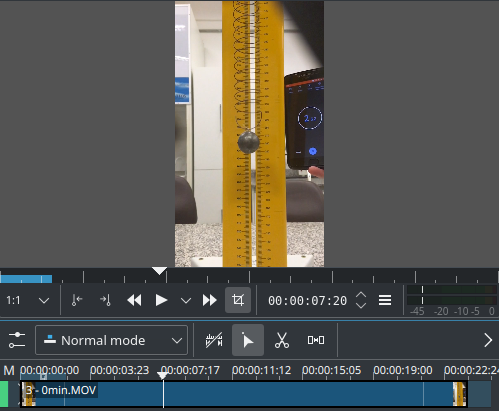
\includegraphics[scale=0.4]{./img/quadros.png}
				\captionsetup{labelformat=empty}
				\caption{\textbf{Figura 3:} Análise da gravação quadro a quadro.}
			\end{figure}
			\begin{figure}[H] \label{img:m1}
				\centering
				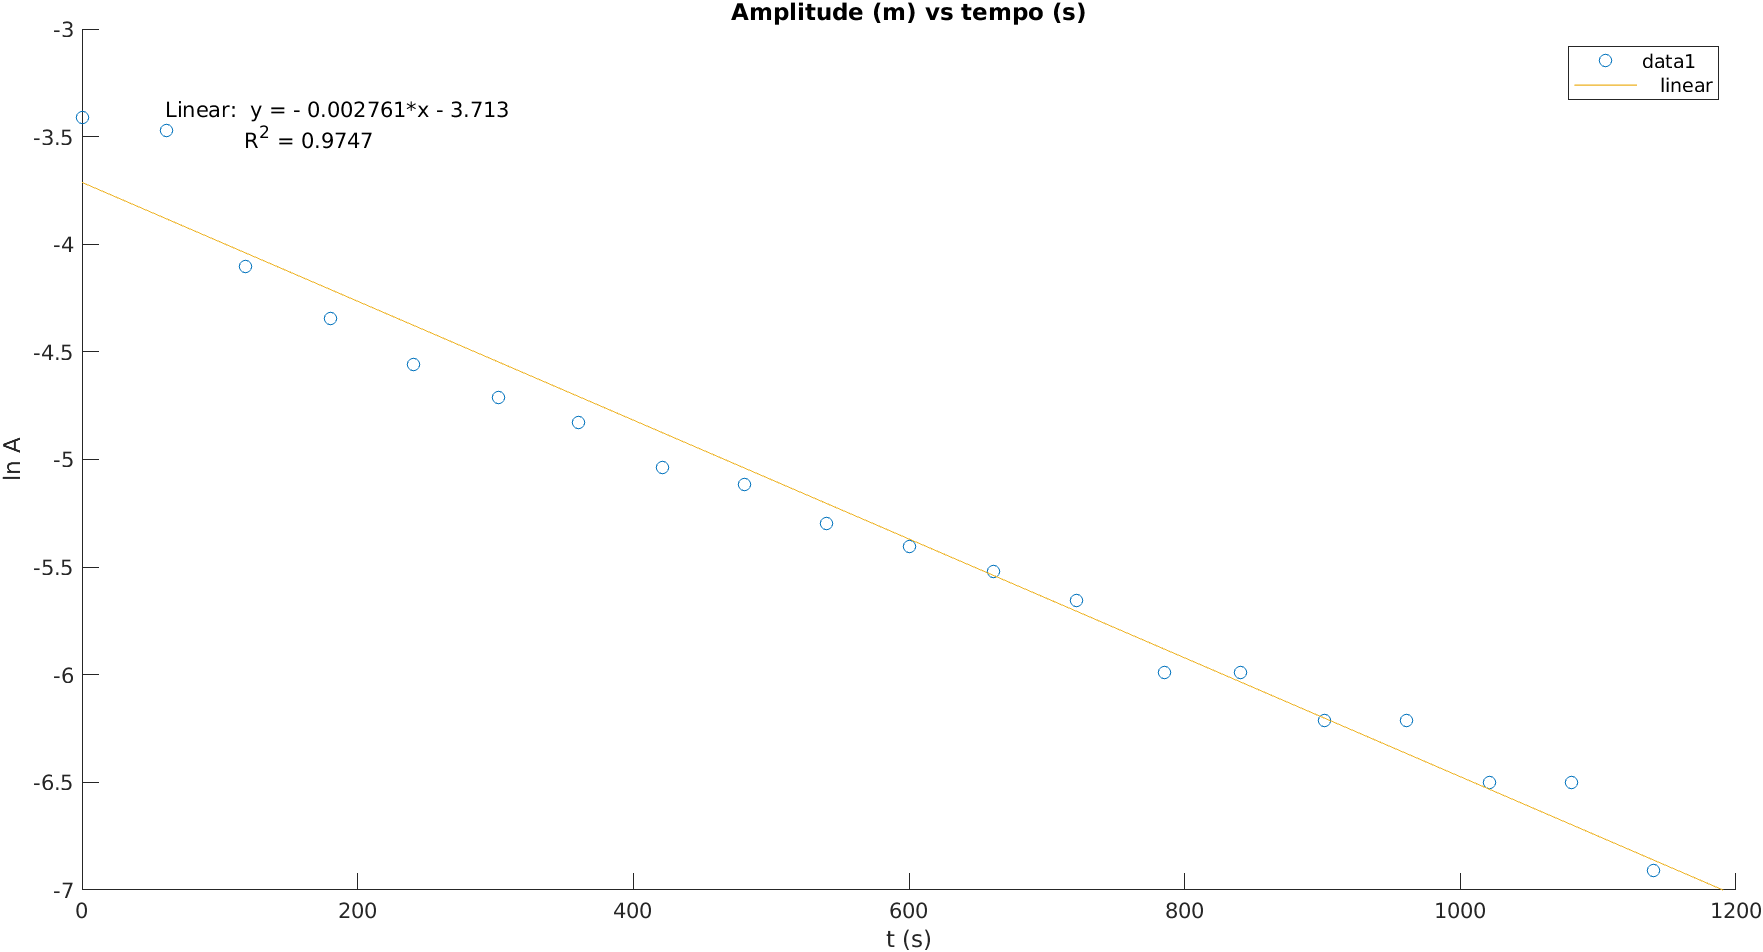
\includegraphics[scale=0.3]{./img/m1.png}
				\captionsetup{labelformat=empty}
				\caption{\textbf{Figura 4:} Gráfico com dados do primeiro método.}
			\end{figure}
			\begin{figure}[H] \label{img:m2}
				\centering
				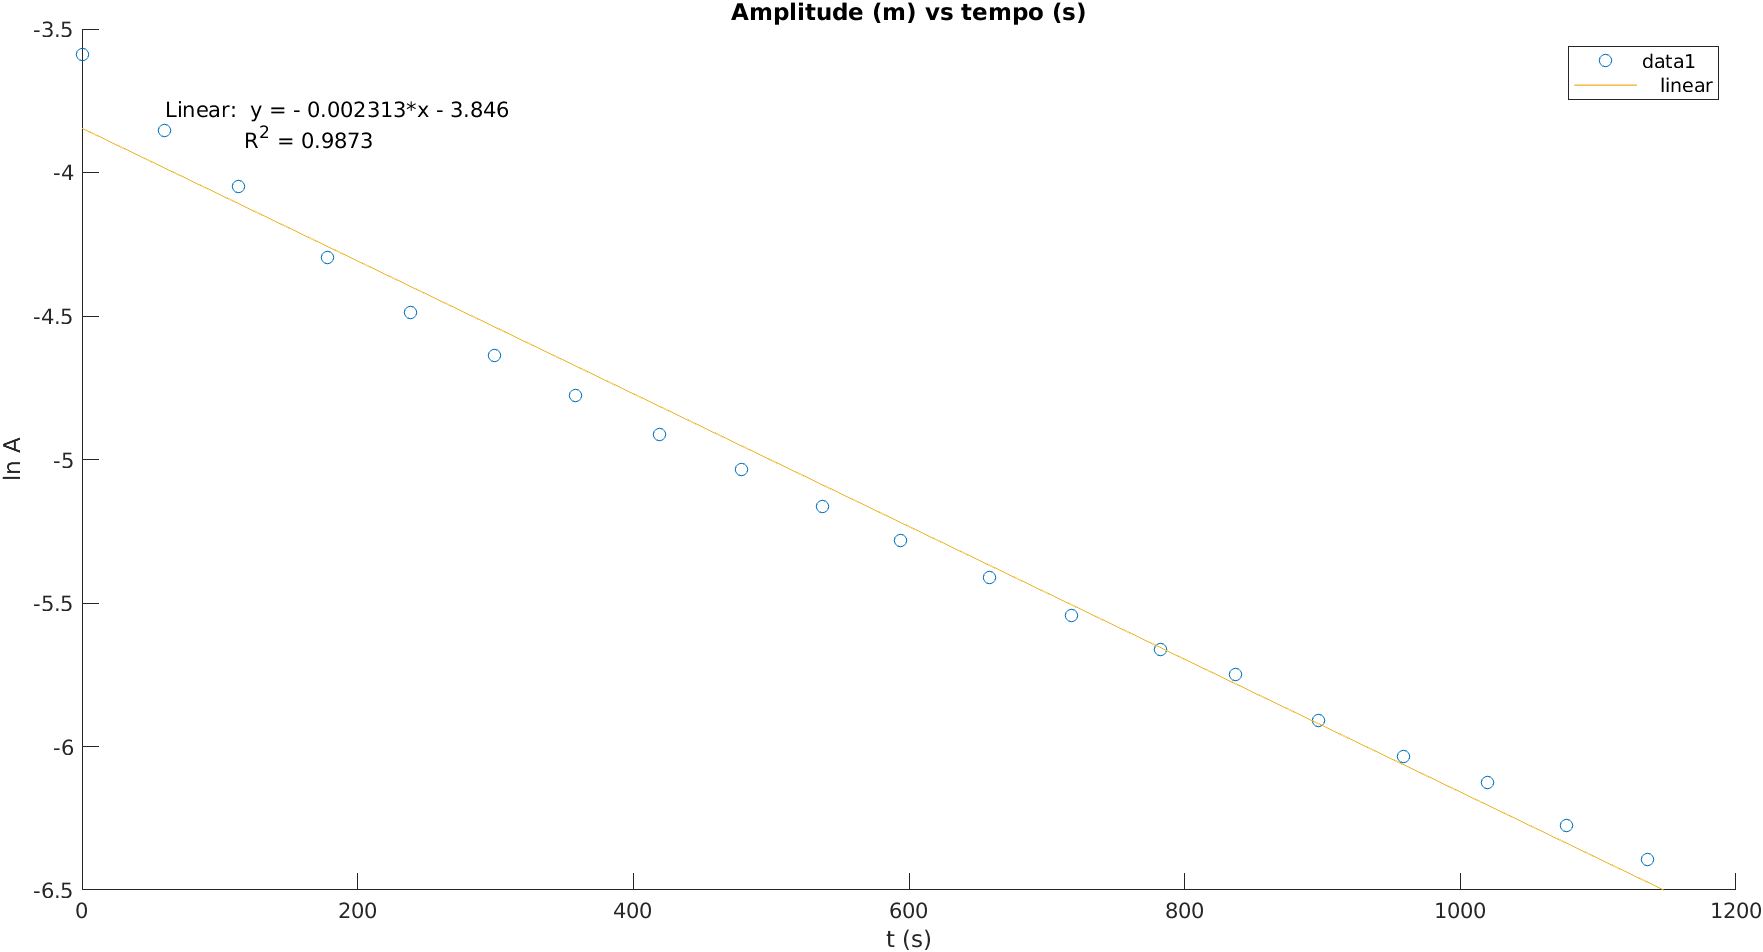
\includegraphics[scale=0.3]{./img/m2.png}
				\captionsetup{labelformat=empty}
				\caption{\textbf{Figura 5:} Gráfico com dados do segundo método.}
			\end{figure}
			\begin{figure}[H] \label{img:m3}
				\centering
				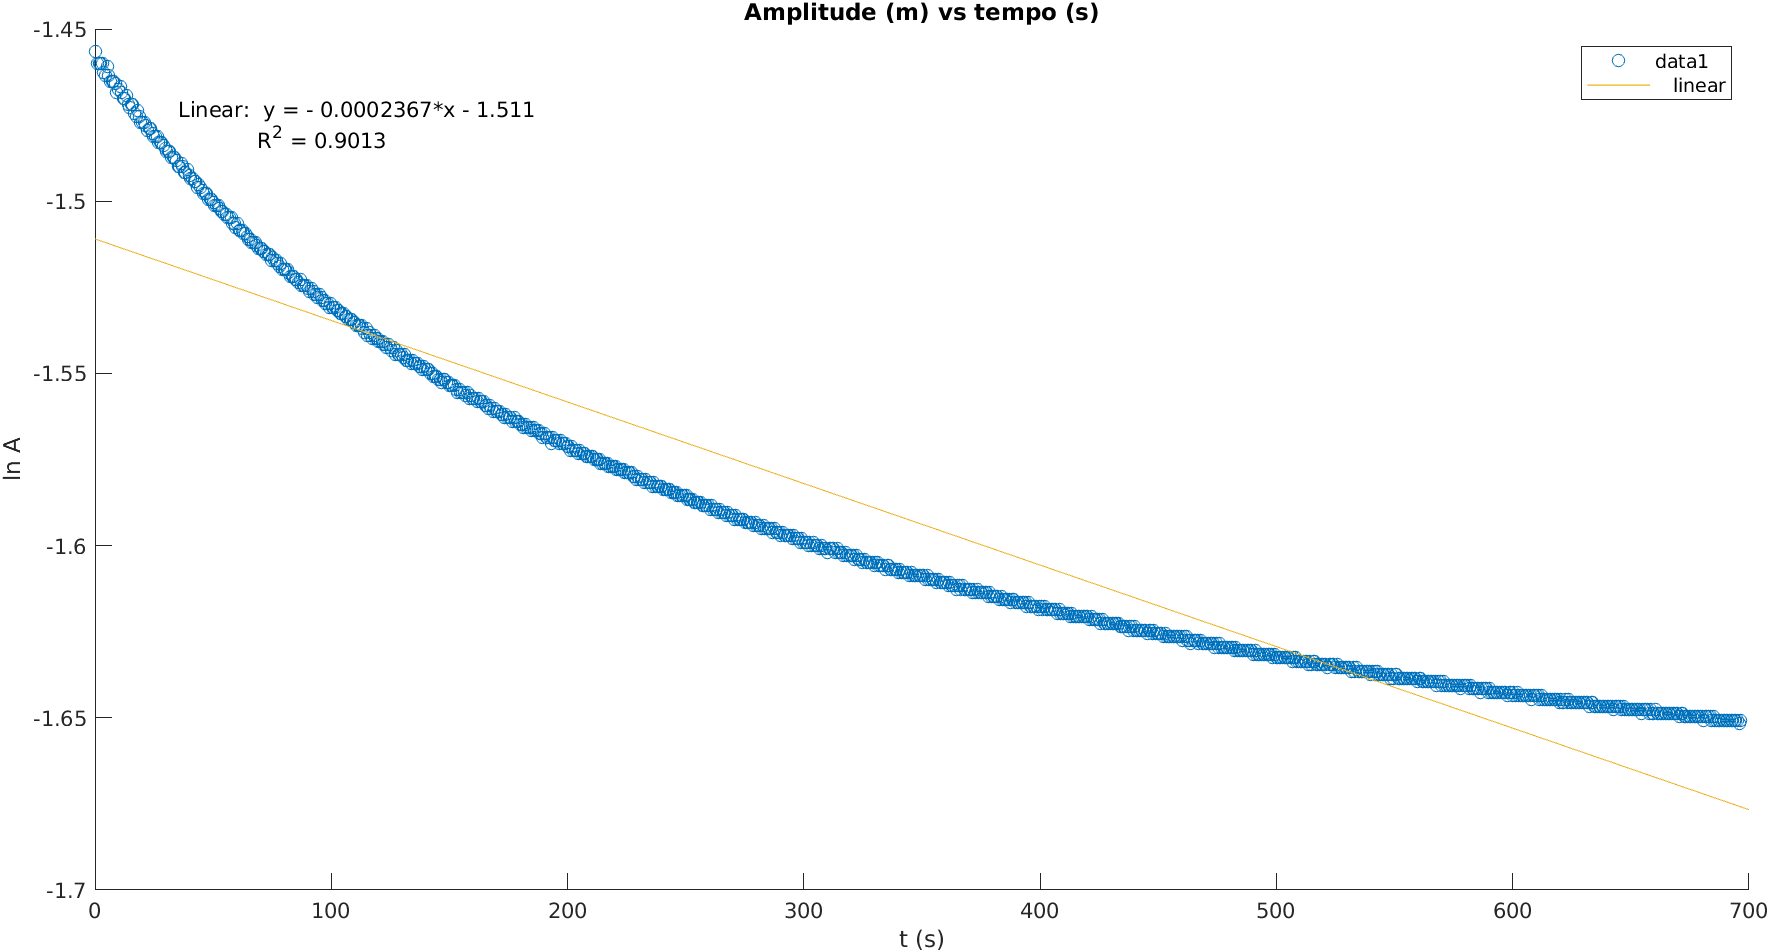
\includegraphics[scale=0.3]{./img/m3.png}
				\captionsetup{labelformat=empty}
				\caption{\textbf{Figura 6:} Gráfico com dados do terceiro método.}
			\end{figure}
			
		\section{Conclusão} \label{sec:conclusao}
		
		\section{Referências}
		
	\end{multicols}
\end{document}
